\documentclass[border=0.2cm]{standalone}
\usepackage[margin=1in]{geometry}
\usepackage{amsmath, amsthm, amssymb, graphicx, multicol, array}
\usepackage{tikz}
\usetikzlibrary{shapes, backgrounds}

\definecolor{blurple}{HTML}{CCCCFF}
\definecolor{mint}{HTML}{CCFFCC}

\begin{document}
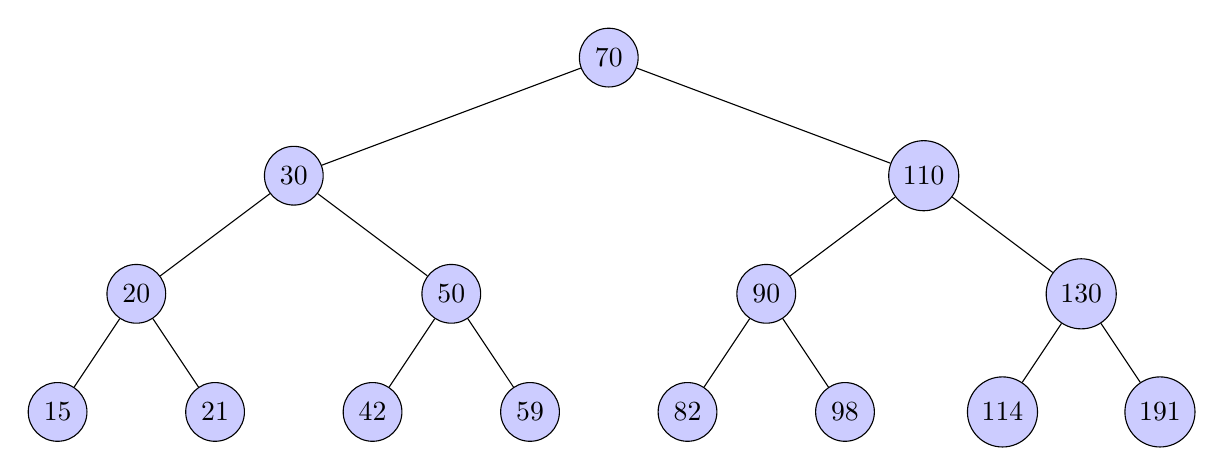
\begin{tikzpicture}[every node/.style={circle, fill=blurple, draw},level 1/.style={sibling distance=80mm},level 2/.style={sibling distance=40mm}, level 3/.style={sibling distance=20mm}, level 4/.style={sibling distance=10mm}]
  \node{70}
  child {node {30}
    child {node {20}
      child {node {15}}
      child {node {21}}}
    child {node {50}
      child {node {42}}
      child {node {59}}}}
  child {node {110}
    child {node {90}
      child {node {82}}
      child {node {98}}}
    child {node {130}
      child {node {114}}
      child {node {191}}}};
\end{tikzpicture}
\end{document}
